
\documentclass[9pt]{beamer}
%\makeatletter
%\def\beamer@calltheme#1#2#3{%
%	\def\beamer@themelist{#2}
%	\@for\beamer@themename:=\beamer@themelist\do
%	{\usepackage[{#1}]{\beamer@themelocation/#3\beamer@themename}}}
%
%\def\usefolder#1{
%	\def\beamer@themelocation{#1}
%}
%\def\beamer@themelocation{}

%\usefolder{../config}

\usetheme[
block=fill,
titleformat=regular,
progressbar=frametitle
]{metropolis}
%\metroset[everytitleformat=regular] % regular, lowercase, uppercase ]
%\metroset[inner/block=fill]

%\setbeameroption{show notes} 
\usepackage{booktabs}
\usepackage[scale=2]{ccicons}

\usepackage{pgfplots}
\usepgfplotslibrary{dateplot}


%\ Hrvatski znakovi
\usepackage[utf8]{inputenc}
\usepackage[T1]{fontenc}
\usepackage[croatian]{babel}
\usepackage{todonotes}
\usepackage{amsmath}
\usepackage{amsfonts}
\selectlanguage{croatian} % american ngerman
\usepackage{todonotes}

% Koristenje Latin modern fonta
% Bez toga na nekim racunalima baca
% err: Font <taj i taj> at <mala velicina, npr4.0pt> not loadable: Metric (TFM) file not found. \end{frame}
\usepackage{lmodern}


\definecolor{RoyalBlue}{cmyk}{1, 0.50, 0, 0}
%\usepackage{natbib}
%\usepackage{bibentry}
\usepackage{scrextend}
\usepackage{hyperref}
%\usepackage[pdfa=true]{hyperref}
\hypersetup{%
    %draft, % = no hyperlinking at all (useful in b/w printouts)
    %colorlinks=true, 
    linktocpage=true, pdfstartpage=3, pdfstartview=FitV,%
    % uncomment the following line if you want to have black links (e.g., for printing)
    %colorlinks=false, linktocpage=false, pdfborder={0 0 0}, pdfstartpage=3, pdfstartview=FitV,% 
    breaklinks=true, pdfpagemode=UseNone, pageanchor=true, pdfpagemode=UseOutlines,%
    plainpages=false, bookmarksnumbered, bookmarksopen=true, bookmarksopenlevel=1,%
    hypertexnames=true, pdfhighlight=/O,%nesting=true,%frenchlinks,%
    %urlcolor=webbrown, linkcolor=RoyalBlue, citecolor=webgreen, %pagecolor=RoyalBlue,%
    %urlcolor=Blue, linkcolor=Blue, citecolor=Red, %pagecolor=Black,%
    %pdftitle={\myTitle},%
    %pdfauthor={\textcopyright\ \myName, \myUni, \myFaculty},%
    pdfsubject={},%
    pdfkeywords={},%
    pdfcreator={pdfLaTeX},%
    pdfproducer={LaTeX with hyperref and classicthesis}, %
    unicode = true 
} 

%\usepackage[pdftex]{graphicx}
% declare the path(s) where your graphic files are
\graphicspath{{./}{./figures/}}


\newcommand{\executeiffilenewer}[3]{%
	\ifnum\pdfstrcmp{\pdffilemoddate{#1}}%
	{\pdffilemoddate{#2}}>0%
	{\immediate\write18{#3}}\fi%
}
\newcommand{\includesvg}[1]{%
	\executeiffilenewer{#1.svg}{#1.pdf}%
	{inkscape -z -C --file=#1.svg %
		--export-pdf=#1.pdf --export-latex}%
	\input{#1.pdf_tex}%
}


% http://tex.stackexchange.com/questions/83882/how-to-highlight-python-syntax-in-latex-listings-lstinputlistings-command

\usepackage{listings}
\usepackage{color}
\usepackage[semibold]{sourcecodepro}

% Default fixed font does not support bold face
\DeclareFixedFont{\ttb}{T1}{txtt}{bx}{n}{12} % for bold
\DeclareFixedFont{\ttm}{T1}{txtt}{m}{n}{12}  % for normal
% Custom colors
\definecolor{deepblue}{rgb}{0,0,0.5}
\definecolor{deepred}{rgb}{0.6,0,0}
\definecolor{deepgreen}{rgb}{0,0.5,0}


% Python style for highlighting
\newcommand\pythonstyle{\lstset{
		language=Python,
		basicstyle=\small\ttfamily,
		otherkeywords={self},             % Add keywords here
		keywordstyle=\small\ttfamily\color{deepblue},
		emph={MyClass,__init__},          % Custom highlighting
		emphstyle=\small\ttfamily\color{deepred},    % Custom highlighting style
		stringstyle=\color{deepgreen},
		frame=tb,                         % Any extra options here
		showstringspaces=false            % 
	}}
	
	
	% Python environment
	\lstnewenvironment{python}[1][]
	{
		\pythonstyle
		\lstset{#1}
	}
	{}
	
	% Python for external files
	\newcommand\pythonexternal[2][]{{
			\pythonstyle
			\lstinputlisting[#1]{#2}}}
	
	% Python for inline
	\newcommand\pythoninline[1]{{\pythonstyle\lstinline!#1!}}

% \includeonlyframes{current}

%\documentclass[ucs]{beamer}
%\usetheme[menuwidth={0.3\paperwidth}]{erlangen}
%\setbeamercovered{transparent=20} 

\usepackage{amsmath,amsfonts,amsthm,amssymb}
\usepackage{setspace}
\usepackage{Tabbing}
\usepackage{fancyhdr}
\usepackage{lastpage}
\usepackage{extramarks}
\usepackage{chngpage}
\usepackage{soul,color}
\usepackage{graphicx,float,wrapfig}
\usepackage{xcolor}
\usepackage[normalem]{ulem}
\usepackage{mathtools}

\definecolor{erlangenlyellow}{RGB}{123, 25, 121}
%\usepackage[utf8x]{inputenc}
%\usepackage{default}
%\usepackage[T1]{fontenc}

\usepackage{verbatim}
\usepackage{listings}


\usepackage{subcaption}
\usepackage{lmodern}

\title{Interpolacije}

\subtitle{ Would such a thing be read and understood so easily?}
\institute{Računalna grafika}


\begin{document}
\begin{frame}
 \titlepage
\end{frame}

%\begin{frame}{Sadržaj}
%  \tableofcontents
%  % You might wish to add the option [pausesections]
%\end{frame}
% \section{Uvod}
\section{Linearna interpolacija}
\begin{frame}{Linearna interpolacija}
	\begin{align*}
	x(t) = x_0 + (x_1-x_0)t
	\end{align*}
	\begin{align*}
	x(t) = (1-t)\cdot x_0 + t\cdot x_1
	\end{align*}
	\begin{align*}
	b_0(t) & = 1-t \\
	b_1(t) & = t
 	\end{align*}
 	\begin{align*}
 	b_0(t) + b_1(t) = 1
 	\end{align*}
 	\hrule\hfill
 	\begin{align*}
 	x(t) = b_0 x_0 + b_1 x_1
 	\end{align*}
\end{frame}
\begin{frame}{Linearna interpolacija}
	Umjereno zanimljivo: $b_0$ i $b_1$ su težinske funkcije, a baricentrične koordinate se mogu izračunati kao omjeri nasuprotne duljine i duljine čitavog segmenta:
	\begin{align*}
	b_0 & = \frac{\textrm{duljina}(x, x_1)}{\textrm{duljina}(x_0, x_1)} \\
	b_1 & = \frac{\textrm{duljina}(x_0, x)}{\textrm{duljina}(x_0, x_1)}
	\end{align*}
	\begin{center}
		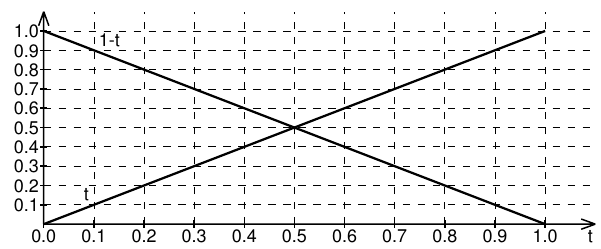
\includegraphics[height=1.5cm]{./slike/lin_interp_01.png}
	\end{center}
\end{frame}
\begin{frame}{Linearna interpolacija vektora}
	\begin{align*}
		\vec{v}(t) = (1-t)\vec{v}_0 + t\vec{v}_1
	\end{align*}
	Interpolira se svaka komponenta vektora zasebno:
	\begin{align*}
		v_x(t) &= (1-t)v_{0,x} + tv_{1,x} \\
		v_y(t) &= (1-t)v_{0,y} + tv_{1,y} \\
		v_z(t) &= (1-t)v_{0,z} + tv_{1,z}
	\end{align*}
	Svojstva interpolacije:
	\begin{itemize}
		\item Kut interpoliranog vektora se postupno mijenja od početnog prema konačnom, no promjena kuta
		nije linearna
		\item Norma interpoliranog vektora može biti neočekivana – primjerice, interpolacijom između vektora
		norme 1 i vektora norme 2 moguće je dobiti vektor norme 0.1
		\item Računska složenost je vrlo niska
	\end{itemize}
\end{frame}
\begin{frame}{Interpolacija kubnim polinomima}
	\begin{align*}
		x(t) = b_0(t) x_0 + b_1(t) x_1
	\end{align*}
	
	\begin{align*}
		b_0(t) &= a_0t^3+b_0t^2+c_0t + d_0
		b_1(t) &= a_1t^3+b_1t^2+c_1t + d_1
	\end{align*}
	Uvjeti:
	\begin{enumerate}
		\item $b_0(t) + b_1(t) = 1$
		\item $b_1(0) = 0$, $b_0(0) = 1$,  $b_1(1) = 1$,$b_0(1) = 0$ 
		\item Derivacije su simetrične: $b'_1(t) = b'_1(1-t)$, $b'_0(t) = b'_0(1-t)$
		\item za $t=1/2$, $b_1(t) = 1-b_1(t)$
	\end{enumerate}
\end{frame}
\begin{frame}{Interpolacija kubnim polinomima}
	Iz ($2$)
	\begin{align*}
	b_1(0)  = 0 & \rightarrow a_1\cdot 0+b_1\cdot 0 +c_1 \cdot 0 + d_1 \\
	            & \rightarrow d_1 = 0 \\
	b_1(1)  = 1 & \rightarrow a_1\cdot 1^3+b_1\cdot 1^2 +c_1 \cdot 1 + d_1 \\
	            & \rightarrow a_1 +b_1  +c_1 + d_1  = 1 \\% \mathrm{ali kako je } $d_1=0$,\\
	            & \rightarrow a_1 +b_1  +c_1   = 1
	\end{align*}
	Iz ($3$)
	\begin{align*}
		b'_1(t) = 3a_1t^2+2b_1 t +c_1
	\end{align*}
	\begin{align*}
		3a_1t^2+2b_1 t +c_1 = 3a_1(1-t)^2+2b_1 (1-t)+c_1
	\end{align*}
	Iz čega se dobije:
	\begin{align*}
		3a_1+2b_1 = 0
	\end{align*}
\end{frame}
\begin{frame}{Interpolacija kubnim polinomima}
	Iz ($4$)
	\begin{align*}
	b_1(1-t) = 1-b_1(t)
	\end{align*}
	Kako već znamo da je $d_1=0$,
	\begin{align*}
		a_1(1-t)^3+b_1(1-t)^2+c_1(1-t) = 1- (a_1t^3+b_1t^2+c_1t)
	\end{align*}
	Ili:
	\begin{align*}
		a_1+b_1 + c_1 = 0
	\end{align*}
\end{frame}
\begin{frame}{Interpolacija kubnim polinomima}
	Rezultat? I dalje tri jednadžbe i četiri nepoznanice:
	\begin{itemize}
		\item $d_1=0$
		\item $3a_1+2b_1 = 0$
		\item $a_1+b_1 + c_1 = 0$
	\end{itemize}
Rješenje? Zadati derivaciju za neki $t$, npr.
\begin{itemize}
	\item $b'_1(0)=0$
	\item $b'_1(0)=1$
	\item $b'_1(0)=1/2$
	\item $b'_1(0)=2$
\end{itemize}
\end{frame}
\begin{frame}{Interpolacija kubnim polinomima}
	$b'_1(0)=0$ \\
	\begin{itemize}
		\item $d_1=0$
		\item $3a_1+2b_1 = 0$
		\item $a_1+b_1 + c_1 = 0$
		\item $c_1=0$
	\end{itemize}
	Rješenje: $a_1=-2$, $b_1=3$, $c_1=0$, $d_1=0$,
	\begin{align*}
		b_1(t) &= -2t^3 + 3t^2 \\
		b_0(t) &= 1-b_1(t) = 1+2t^3 - 3t^2
	\end{align*}
\begin{center}
	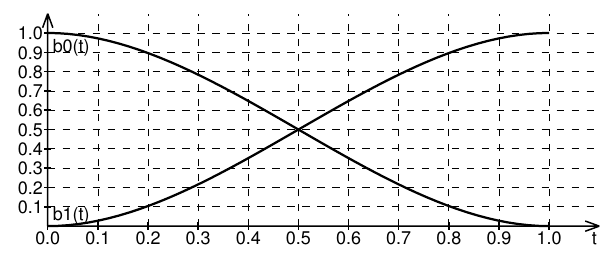
\includegraphics[height=2.5cm]{./slike/lin_interp_der_eq_0.png}
\end{center}
\end{frame}

\begin{frame}{Bilinearna interpolacija}
	Tražimo vrijednost $f$ u točki $(x, y)$ dok su poznate vrijednosti $Q11 = (x1, y1), Q12 = (x1, y2), Q21 = (x2, y1), and Q22 = (x2, y2)$. 
	\begin{center}
		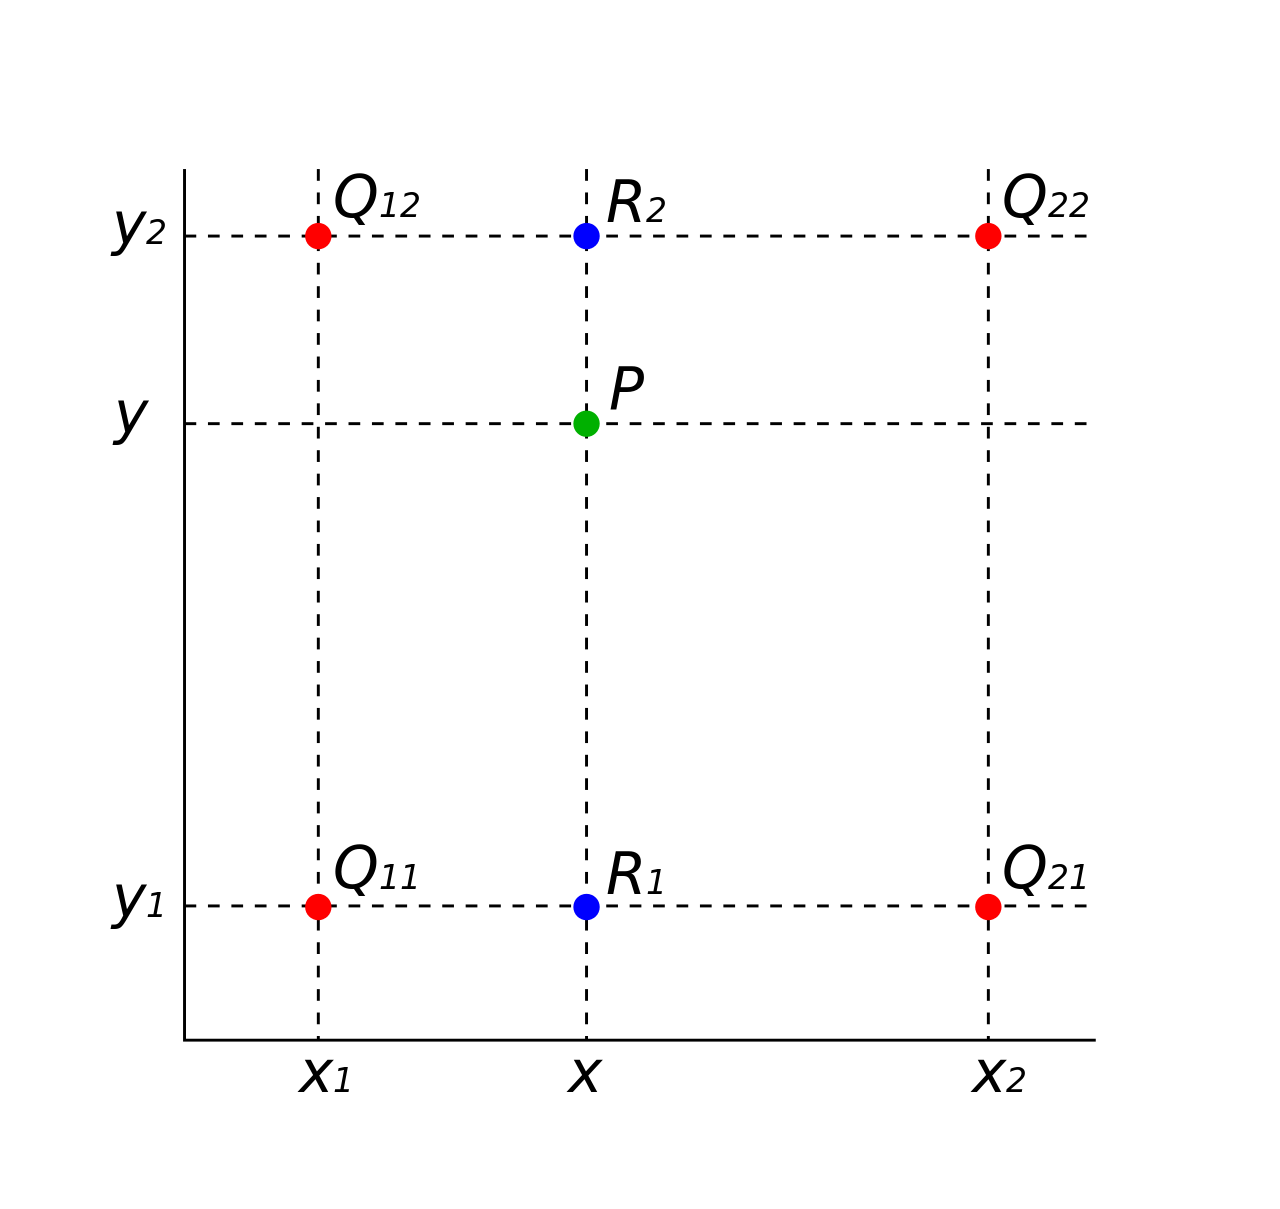
\includegraphics[height=2.5cm]{./slike/bilinear_interpolation.png}
	\end{center}
	Interpoliramo u $x$ smjeru:
	\begin{align*}
	f(x, y_1) & \approx \frac{x_2 - x}{x_2 - x_1} f(Q_{11}) + 
	            \frac{x - x_1}{x_2 - x_1} f(Q_{21}) \\
	f(x, y_2) & \approx \frac{x_2 - x}{x_2 - x_1} f(Q_{12}) + 
	            \frac{x - x_1}{x_2 - x_1} f(Q_{22})
	\end{align*}
	A onda i u $y$ smjeru:
	\begin{align*}
		f(x, y) & \approx \frac{y_2 - y}{y_2 - y_1} f(x, y_1) +
		           \frac{y - y_1}{y_2 - y_1} f(x, y_2)
	\end{align*}
\end{frame}
\begin{frame}{Bilinearna interpolacija}
	\begin{center}
		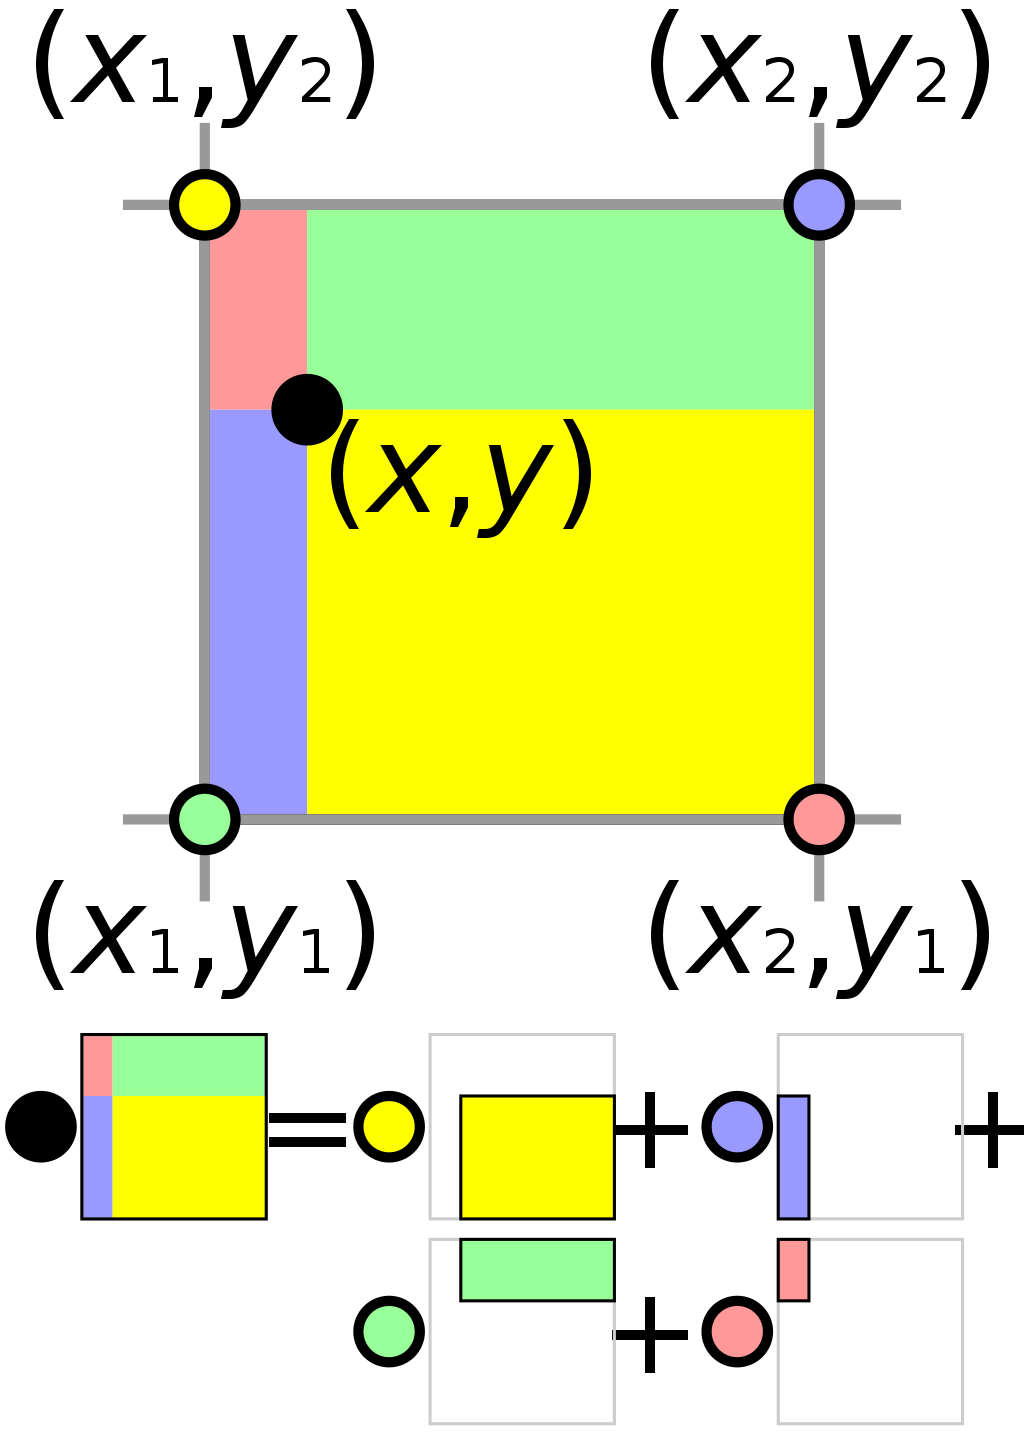
\includegraphics[height=5.5cm]{./slike/bilinear_interpolation_2.png}
	\end{center}
\end{frame}

\begin{frame}{Interpolacija trokuta}
	\begin{center}
		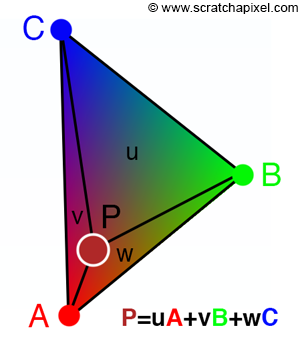
\includegraphics[height=5.5cm]{./slike/barycentriccolor.png}
	\end{center}
\end{frame}

\begin{frame}{Neke klasifikacije  i svojstva krivulja}
	\begin{itemize}
		\item periodičke $\leftrightarrow$ neperiodičke
		\item racionalne $\leftrightarrow$ neracionalne
		\item otvorene $\leftrightarrow$ zatvorene
	\end{itemize}
	\begin{itemize}
		\item Mogucnost prikaza višestrukih vrijednosti (za jedan x više mogucih y vrijednosti - nekada poželjnom nekada i ne baš).
		\item Nezavisnost od koordinatnog sustava.
		\item Svojstvo lokalnog nadzora (promjena jedne tocke uzrokuje promjenu oblika krivulje samo u 	okolini te tocke).
		\item Smanjenje varijacije (što manje oscilacija).
		\item Red neprekidnosti što veći.
		\item Mogucnost opisa osnovnih geometrijskih oblika (kružnica, elipsa \ldots )
	\end{itemize}	
\end{frame}	
\section{O linijama}
\begin{frame}{Svojstva neprekidnutosti linija}
	\begin{itemize}
		\item<1-> $C^{0}$ kontinuirana linija
		\item<2-> $C^{1}$ prva derivacija kontinuirana, neprekinuta
		\item<3-> $C^{2}$ druga derivacija neprekinuta, neprekinuta zakrivljenost
		\item<4-> $G^{1}$ geometrijska neprekinutost, tangente u istom smjeru
	\end{itemize}
	\begin{center}
		\only<1>{
			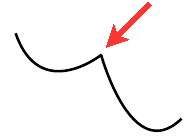
\includegraphics[height=1.5cm]{./slike/c0.png}
		}
		\only<2>{
			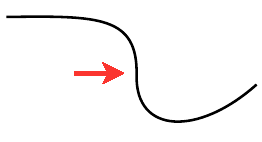
\includegraphics[height=1.5cm]{./slike/c1.png}
		}
		\only<4>{
			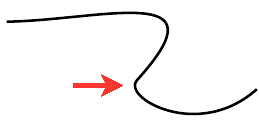
\includegraphics[height=1.5cm]{./slike/g1.png}
		}
	\end{center}
	\only<5>{
		\begin{itemize}
			\item $G^{1}$ - dovoljno dobro za modeliranje
			\item $C^{1}$ - često potrebno za animaciju
		\end{itemize}
	}
\end{frame}
\begin{frame}{Parametarski oblik funkcije}
	\begin{itemize}
		\item rezultat linearne interpolacije
	\end{itemize}
	Odrediti točku na 20\% udaljenosti od prve točke:
	\begin{align*}
		udaljenost = (p_{2} - p_{1}), \\
		omjer = \frac{postotak}{100}, \\
		p_{0.2} = p_{1} + udaljenost \cdot omjer
	\end{align*}
	Ovjde je $omjer$ zamijenimo s parametrom $t$ o odredimo $0 \leq t \leq 1$
	
\end{frame}
\begin{frame}{Parametarski oblik funkcije}
	\begin{itemize}
		\item oblik parametarske funkcije
	\end{itemize}
	\begin{align*}
		y = \sqrt{1-x^2} \\
		y^2+x^2 = 1
	\end{align*}
	\begin{align*}
		f(a) = \sin(a)\\
		f(b) = \cos(b)
	\end{align*}
	\begin{align*}
		\left \{ \begin{matrix}
			f_a(t) = \sin(t) \\
			f_b(t) = \cos(t)
		\end{matrix} \right.
	\end{align*}
	\begin{align*}
		\left \{ \begin{matrix}
			x = \sin(t) \\
			y = \cos(t)
		\end{matrix} \right.
	\end{align*}
\end{frame}

\begin{frame}{Parametarski oblik kružnice}
	Kružnica:
	\begin{align*}
		\left \{ \begin{matrix}
			x = R\sin(t) + x_c \\
			y = R\cos(t) + y_c
		\end{matrix} \right.
	\end{align*}
\end{frame}	
\begin{frame}{Jednostavna gibanja}
	Osnovni parametri:
	\begin{itemize}
		\item Linearno gibanje po x osi: 
	\end{itemize}
	$$(x,y,z) = f(t) = (t,0,0)$$
	\begin{itemize}
		\item Gibanje po sinusoidi: 
	\end{itemize}
	$$(x,y,z) = f(t) = (t,sin(t),0)$$
	
	\begin{itemize}
		\item Promjena boje  - od crne do žute: 
	\end{itemize}
	$$(r,g,b) = f(t) = (t,t,0)$$
\end{frame}

\begin{frame}{Još primjera:}
	Osnovni parametri:
	\begin{itemize}
		\item Gibanje po kružnici: 
	\end{itemize}
	$$(x,y,z) = f(t) = (\cos(t),\sin(t),0)$$
	\begin{itemize}
		\item Gibanje po zavojnici: 
	\end{itemize}
	$$(x,y,z) = f(t) = (\cos(t),\sin(t),t)$$
	
	\begin{itemize}
		\item oscilacije: 
	\end{itemize}
	$$(x,y,z) = f(t) = (\sin(t),0,0)$$
	
	\begin{itemize}
		\item njihalo: 
	\end{itemize}
	$$(\phi, r_x,r_y,r_z) = f(t) = (\cos(t),0,0,1)$$
\end{frame}
\section{B\'{e}zier spline}
\begin{frame}{B\'{e}zier spline}
	\only<1>{\begin{itemize}
			\item polinomi:
		\end{itemize}
		\begin{align*}
			f(x) = a \cdot x^3 + b \cdot x^2 + c \cdot x + d
	\end{align*}}
	\only<2->{
		B\'{e}zier spline krivulja je polinomna funkcija od $t$, gdje je $0 \leq t \leq1$
		\begin{align*}
			\mathrm{linearni} &= \quad (1-t) + t \\
			\mathrm{kvadratni} &= (1-t)^2 + 2 \cdot (1-t) \cdot t + t^2 \\
			\textrm{kubični} &= (1-t)^3 + 3 \cdot (1-t)^2 \cdot t + 3 \cdot (1-t) \cdot t^2 + t^3
		\end{align*}
		binomni koeficijenti:
		\begin{align*}
			\mathrm{linearni} &=  \; \; \;\; \; \;\; \; \; 1 + 1 \\
			\mathrm{kvadratni} &=  \; \; \; \; \; \;1  + 2 + 1 \\
			\textrm{kubični} &=  \; \; \; 1 + 3 + 3 + 1\\
			\mathrm{4. red} &= 1 + 4 + 6 + 4 + 1
		\end{align*}
	}
\end{frame}

\begin{frame}{B\'{e}zier spline}
	Ako postavimo $a = 1-t$ i $b = t:$
		\begin{align*}
		\mathrm{linearni} &= {\color{blue}a} + {\color{red}b} \\
		\mathrm{kvadratni} &= {\color{blue}a} \cdot {\color{blue}a} + {\color{blue}a} \cdot {\color{red}b} + {\color{red}b} \cdot {\color{red}b} \\
		\textrm{kubični} &= {\color{blue}a} \cdot {\color{blue}a} \cdot {\color{blue}a} + {\color{blue}a} \cdot {\color{blue}a} \cdot {\color{red}b} + {\color{blue}a} \cdot {\color{red}b} \cdot {\color{red}b} + {\color{red}b} \cdot {\color{red}b} \cdot {\color{red}b}\\
		\end{align*}

		Opća formula:
		\begin{align*}
		Bezier(n,t) = \sum_{i=0}^{n}
		\underset{binomni\ član}{\underbrace{\binom{n}{i}}}
		\cdot\
		\underset{polinomni\ član}{\underbrace{(1-t)^{n-i} \cdot t^{i}}}
		\end{align*}
	
\end{frame}
\begin{frame}{Intermezzo - binomni član}
	\begin{align*}
	\binom{n}{i} = \frac{n!}{i!(n-i)!} = \frac{n(n-1)(n-2)\ldots (n-i+1)}{i(i-1)(i-2)\ldots 1}
	\end{align*}
	Primjer:
	\begin{align*}
	\binom{7}{4} = \frac{7!}{4!(7-3)!} = \frac{7(7-1)(7-2)(7-3)}{4(4-1)(4-2)(4-3)1} 
	= \frac{7\cdot 6\cdot 5\cdot 4}{4\cdot 3\cdot 2\cdot 1} = 35
	\end{align*}
\end{frame}

\begin{frame}{B\'{e}zier spline}
	Ako je potrebno promijeniti polinom, može se dodavanjem težinskih faktora na svaki polinomni član:
		\begin{align*}
		Bezier(n,t) = \sum_{i=0}^{n}
		\underset{binomni\ član}{\underbrace{\binom{n}{i}}}
		\cdot\
		\underset{polinomni\ član}{\underbrace{(1-t)^{n-i} \cdot t^{i}}}
		\cdot\
		\underset{težinski faktor}{\underbrace{w_i}}
		\end{align*}
	
	
		Težinski faktori $w_{i}$ su koordinate točaka.\\
		Neka su zadane $4$ $2$-d točke $w_i = (x_i,y_i)$:\\
		$w_0 = (120, 160)$, $w_1 = (35, 200)$, $w_2 = (220, 260)$ i $w_3 = (120, 40)$
		\begin{align*}
		\left \{ \begin{matrix}
		x = {\color{blue}120} \cdot (1-t)^3 + {\color{blue}35} \cdot 3 \cdot (1-t)^2 \cdot t + {\color{blue}220} \cdot 3 \cdot (1-t) \cdot t^2 + {\color{blue}220} \cdot t^3 \\
		y = {\color{blue}160} \cdot (1-t)^3 + {\color{blue}200} \cdot 3 \cdot (1-t)^2 \cdot t + {\color{blue}260} \cdot 3 \cdot (1-t) \cdot t^2 + {\color{blue}40} \cdot t^3
		\end{matrix} \right.
		\end{align*}
\end{frame}
\begin{frame}{B\'{e}zier spline}

		\begin{align*}
		B(t) = P_1 \cdot (1-t)^3 + P_2 \cdot 3 \cdot (1-t)^2 \cdot t + P_3 \cdot 3 \cdot (1-t) \cdot t^2 + P_4 \cdot t^3
		\end{align*}
		
		\begin{align*}
		B(t) = (1-t)^3 + 3 \cdot (1-t)^2 \cdot t + 3 \cdot (1-t) \cdot t^2 + t^3
		\end{align*}
		
%		\begin{align*}
%		\begin{matrix}
%		... & = & (1-t)^3 \\
%		& + & 3 \cdot (1-t)^2 \cdot t \\
%		& + & 3 \cdot (1-t) \cdot t^2 \\
%		& + & t^3 \\
%		\end{matrix}
%		\end{align*}
%		\begin{align*}
%		\begin{matrix}
%		... & = & ( -t^3 + 3 \cdot t^2 - 3 \cdot t + 1) \\
%		& + & (3 \cdot t^3 - 6 \cdot t^2 + 3 \cdot t) \\
%		& + & (-3 \cdot t^3 + 3 \cdot t^2) \\
%		& + & (t^3) \\
%		\end{matrix}
%		\end{align*}

	\begin{align*}
		... & \begin{matrix}
		& = & (1-t)^3 \\
		& + & 3 \cdot (1-t)^2 \cdot t \\
		& + & 3 \cdot (1-t) \cdot t^2 \\
		& + & t^3 \\
		\end{matrix} \\ 
		... & 
		\begin{matrix}
		& = & ( -t^3 + 3 \cdot t^2 - 3 \cdot t + 1) \\
		& + & (3 \cdot t^3 - 6 \cdot t^2 + 3 \cdot t) \\
		& + & (-3 \cdot t^3 + 3 \cdot t^2) \\
		& + & (t^3) \\
		\end{matrix}
	\end{align*}
\end{frame}

\begin{frame}{B\'{e}zier spline}
	\only<1-2>{
		\begin{align*}
		\begin{matrix}
		... & = & ( -t^3 + 3 \cdot t^2 - 3 \cdot t + 1) \\
		& + & (3 \cdot t^3 - 6 \cdot t^2 + 3 \cdot t) \\
		& + & (-3 \cdot t^3 + 3 \cdot t^2) \\
		& + & (t^3) \\
		\end{matrix}
		\end{align*}}
	\onslide<2->{\begin{align*}
		\begin{matrix}
		... & = & -1 \cdot t^3 + 3 \cdot t^2 - 3 \cdot t + 1 \\
		& + & +3 \cdot t^3 - 6 \cdot t^2 + 3 \cdot t + 0 \\
		& + & -3 \cdot t^3 + 3 \cdot t^2 + 0 \cdot t + 0 \\
		& + & +1 \cdot t^3 + 0 \cdot t^2 + 0 \cdot t + 0 \\
		\end{matrix}
		\end{align*}}
	\onslide<3->{
		\begin{align*}
		\begin{bmatrix}t^3 & t^2 & t & 1\end{bmatrix} \cdot \begin{bmatrix*}[r]-1 \\ 3 \\ -3 \\ 1\end{bmatrix*}
		+ \begin{bmatrix}t^3 & t^2 & t & 1\end{bmatrix} \cdot \begin{bmatrix*}[r]3 \\ -6 \\ 3 \\ 0\end{bmatrix*}\\
		+ \begin{bmatrix}t^3 & t^2 & t & 1\end{bmatrix} \cdot \begin{bmatrix*}[r]-3 \\ 3 \\ 0 \\ 0\end{bmatrix*}
		+ \begin{bmatrix}t^3 & t^2 & t & 1\end{bmatrix} \cdot \begin{bmatrix*}[r]1 \\ 0 \\ 0 \\ 0\end{bmatrix*}
		\end{align*}}
\end{frame}

\begin{frame}{B\'{e}zier spline}
	\onslide<1->{\begin{align*}
		\begin{bmatrix}t^3 & t^2 & t & 1\end{bmatrix} \cdot 
		\begin{bmatrix*}[r]
		-1 &  3 & -3 & 1 \\
		3 & -6 &  3 & 0 \\
		-3 &  3 &  0 & 0 \\
		1 &  0 &  0 & 0
		\end{bmatrix*}
		\end{align*}}
	\onslide<2->{
		\begin{align*}
		\begin{bmatrix}1 & t & t^2 & t^3\end{bmatrix} \cdot 
		\begin{bmatrix*}[r]
		1 &  0 &  0 & 0 \\
		-3 &  3 &  0 & 0 \\
		3 & -6 &  3 & 0 \\
		-1 &  3 & -3 & 1
		\end{bmatrix*}
		\end{align*}
	}
	\onslide<3->{
		\begin{align*}
		B(t) = \begin{bmatrix}
		1 & t & t^2 & t^3
		\end{bmatrix}
		\cdot
		\begin{bmatrix*}[r]
		1 &  0 &  0 & 0 \\
		-3 &  3 &  0 & 0 \\
		3 & -6 &  3 & 0 \\
		-1 &  3 & -3 & 1
		\end{bmatrix*}
		\cdot
		\begin{bmatrix}
		P_1 \\ P_2 \\ P_3 \\ P_4
		\end{bmatrix}
		\end{align*}
	}
\end{frame}

\begin{frame}{B\'{e}zier spline}
	\begin{itemize}
		\item Kubični B\'{e}zierov spline
	\end{itemize}
	\begin{align*}
	B(t) = \begin{bmatrix}
	1 & t & t^2 & t^3
	\end{bmatrix}
	\cdot
	\begin{bmatrix}
	1 &  0 &  0 & 0 \\
	-3 &  3 &  0 & 0 \\
	3 & -6 &  3 & 0 \\
	-1 &  3 & -3 & 1
	\end{bmatrix}
	\cdot
	\begin{bmatrix}
	P_1 \\ P_2 \\ P_3 \\ P_4
	\end{bmatrix}
	\end{align*}
	
	\begin{itemize}
		\item Kvadratni B\'{e}zierov spline
	\end{itemize}
	\begin{align*}
	B(t) = \begin{bmatrix}
	1 & t & t^2
	\end{bmatrix}
	\cdot
	\begin{bmatrix}
	1 &  0 & 0 \\
	-2 &  2 & 0 \\
	1 & -2 & 1
	\end{bmatrix}
	\cdot
	\begin{bmatrix}
	P_1 \\ P_2 \\ P_3
	\end{bmatrix}
	\end{align*}
\end{frame}

\begin{frame}{B\'{e}zier spline}
	Kao u skripti:
	\begin{align*}
	B(t) = \mathbf{T}\mathbf{B}\mathbf{R}
	\end{align*}
\end{frame}

\begin{frame}{B\'{e}zier spline, rekurzivni algoritam}
	\begin{block}{Trik}
		Razdijeliti domenu na dvije polovice. Onda svaku polovicu na dvije polovice, itd. 
		
		Korisno kod crtanja.
	\end{block}
	\begin{itemize}
		\item Odabire se novi parametar za kojeg vrijedi $t = \lambda/2$ 
	\end{itemize}	
	\begin{align*}
	B(t) &= \begin{bmatrix}
	\left(\frac{\lambda}{2}\right)^2 & \frac{\lambda}{2} & 1 
	\end{bmatrix}\mathbf{B}\mathbf{R} \\
	&= \begin{bmatrix}
	\lambda^2 & \lambda & 1 
	\end{bmatrix} 
	\begin{bmatrix}
	\left(\frac{1}{2}\right)^2 &  0 & 0 \\
	0 &  \left(\frac{1}{2}\right)^1 & 0 \\
	0 & 0 & \left(\frac{1}{2}\right)^0
	\end{bmatrix}
	\mathbf{B}\mathbf{R} \\
	&= \mathbf{\lambda}\mathbf{L}\mathbf{B}\mathbf{R} \\
	&= \mathbf{\lambda}\mathbf{B}(\mathbf{B}^{-1}\mathbf{L}\mathbf{B}\mathbf{R})
	=  \mathbf{\lambda}\mathbf{B}\mathbf{R}_L
	\end{align*}
\end{frame}

\section{Derivacije B\'{e}zierove spline krivulje}
\begin{frame}{Derivacije}
	\begin{align*}
	Bezier'(n,t) = n \cdot \sum_{i=0}^{n-1} (b_{i+1}-b_i) \cdot Bezier(n-1,t)_i 
	\end{align*}
	\begin{align*}
	Bezier'(n,t) = \sum_{i=0}^{n-1} Bezier(n-1,t)_i \cdot n \cdot (w_{i+1}-w_i)
	\end{align*}
	Derivacija B\'{e}zierove spline krivulje $n$-tog reda jest B\'{e}zierova spline krivulja $n-1$ reda s novim težinskim koeficijentima $w'_{0}\ldots w'{n-1}$ izvedenim iz pretkodnih koeficijenata $w_{0}\ldots w_{n}$
	
	
\end{frame}

\begin{frame}{Derivacije}
	\begin{align*}
	Bezier(n,t) = \sum_{i=0}^{n}
	\underset{binomni\ clan}{\underbrace{\binom{n}{i}}}
	\cdot\
	\underset{polinomni\ clan}{\underbrace{(1-t)^{n-i} \cdot t^{i}}}
	\cdot\
	\underset{tez.\ faktor}{\underbrace{w_i}}
	\end{align*}
	\begin{align*}
	Bezier'(n,t) = \sum_{i=0}^{k}
	\underset{binomni\ clan}{\underbrace{\binom{k}{i}}}
	\cdot\
	\underset{polinomni\ clan}{\underbrace{(1-t)^{k-i} \cdot t^{i}}}
	\cdot\
	\underset{tez.\ faktor}{\underbrace{n \cdot (w_{i+1} - w_i)}}
	{}
	\end{align*}
	Ovdje je $k = n -1 $
\end{frame}

\begin{frame}{Primjer}
	\begin{align*}
	B(n, t),    & n = 4,  w   =\{w_1,  w_2,   w_3, w_4\} \\	
	B'(n, t),   & n = 3,  w'  =\{w'_1,  w'_2, w'_3    \} = \{3(w_2 -w_1),  3(w_3 -w_2), 3(w_4-w_3)\} \\
	B''(n, t),  & n = 2,  w'' =\{w''_1, w''_2         \} = \{2(w'_2-w'_1), 2(w'_3-w'_2)\} \\
	B'''(n, t), & n = 1,  w'''=\{w'''_1               \} = \{(w''_2-w''_1)\}
	\end{align*}
\end{frame}

\begin{frame}{tangente i normale}
	\begin{itemize}
		\item tangente su jednostavne
	\end{itemize}
	\begin{align*}
	\left \{ \begin{matrix}
	tangent_x(t) = B'_x(t) \\
	tangent_y(t) = B'_y(t)
	\end{matrix} \right.
	\end{align*}
	\begin{align*}
	d = || tangent(t) || = \sqrt{B'_x(t)^2 + B'_y(t)^2}
	\end{align*}
	\begin{align*}
	\left \{ \begin{matrix}
	\hat{x}(t) = || tangent_x(t) ||
	=\frac{tangent_x(t)}{ || tangent(t) || }
	= \frac{B'_x(t)}{d} \\
	\hat{y}(t) = || tangent_y(t) ||
	= \frac{tangent_y(t)}{ || tangent(t) || }
	= \frac{B'_y(t)}{d}
	\end{matrix} \right.
	\end{align*}
\end{frame}
\begin{frame}{tangente i normale}
	
	\begin{align*}
	\left \{ \begin{array}{l}
	normal_x(t) = \hat{x}(t) \cdot \cos{\frac{\pi}{2}} - \hat{y}(t) \cdot \sin{\frac{\pi}{2}} = - \hat{y}(t) \\
	normal_y(t) = \underset{rotacija\ za\ 1/4\ kruga} {\underbrace{ \hat{x}(t) \cdot \sin{\frac{\pi}{2}} + \hat{y}(t) \cdot \cos{\frac{\pi}{2}} }} = \hat{x}(t)
	\end{array} \right.
	\end{align*}
	
	\begin{align*}
	\begin{array}{l}
	x' = x \cdot \cos(\phi) - y \cdot \sin(\phi) \\
	y' = x \cdot \sin(\phi) + y \cdot \cos(\phi)
	\end{array}
	\end{align*}
	\begin{align*}
	\begin{bmatrix}
	x' \\ y'
	\end{bmatrix}
	=
	\begin{bmatrix}
	\cos(\phi) & -\sin(\phi) \\
	\sin(\phi) & \cos(\phi)
	\end{bmatrix}
	\begin{bmatrix}
	x \\ y
	\end{bmatrix}
	\end{align*}
\end{frame}

\section{Interpolacijska B\'{e}zierova spline krivulja}
\begin{frame}{B\'{e}zier krivulja s više od 4 točke}
	\begin{center}
		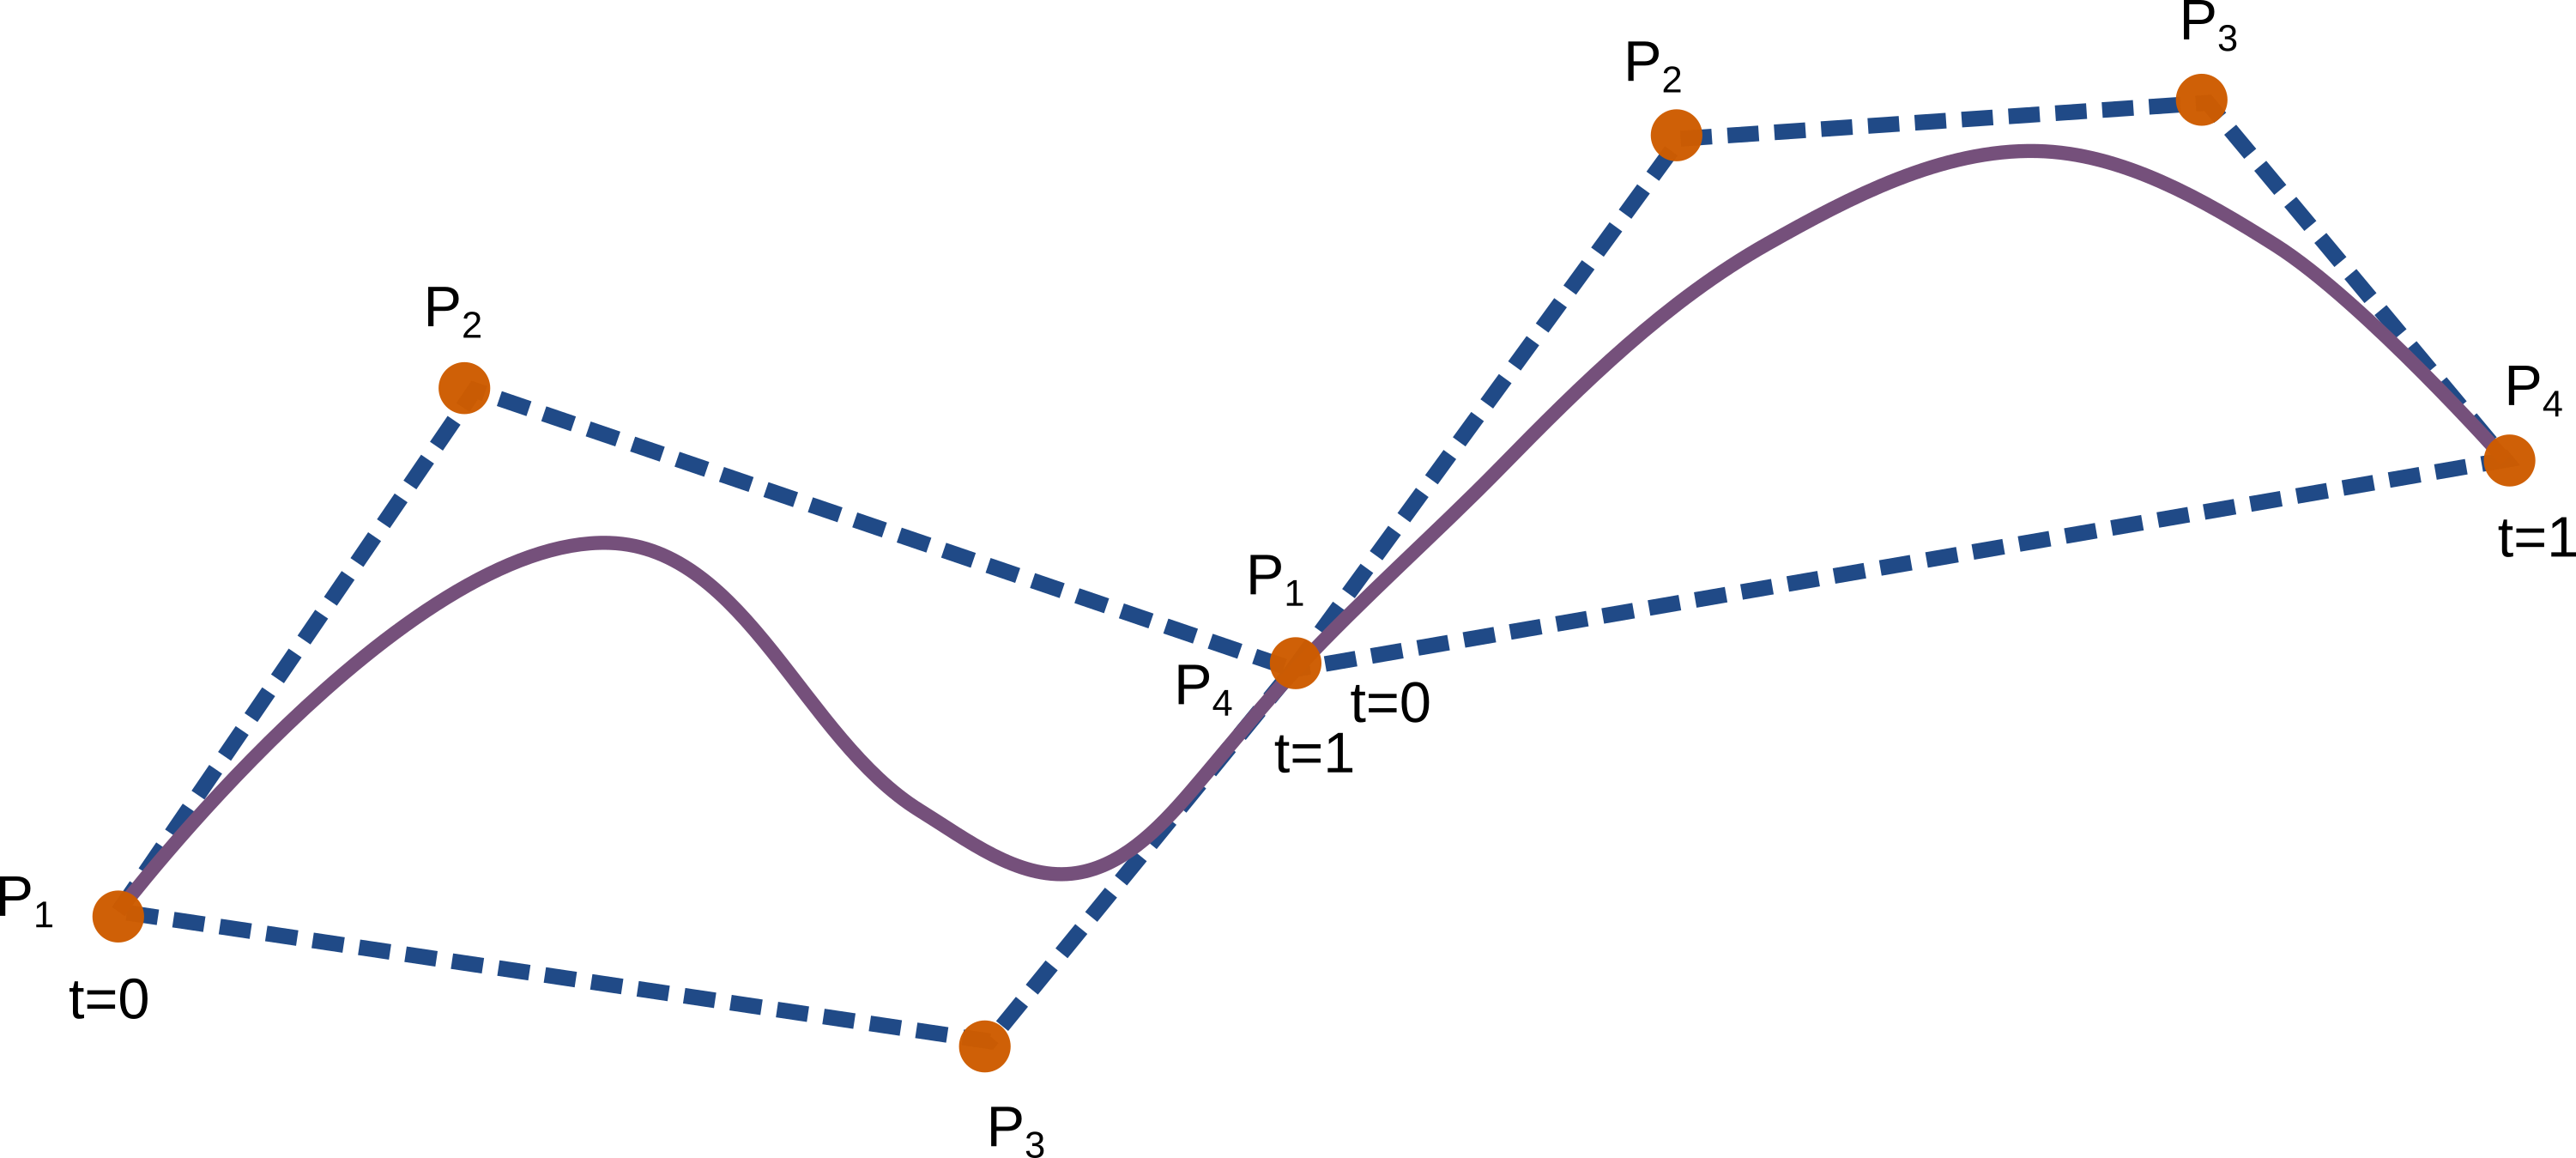
\includegraphics[height=1.5cm]{./slike/bez_vise_od_4.png}
	\end{center}
	\begin{itemize}
		\item Kako garantirati $C^{0}$
		\item Kako garantirati $G^{1}$
		\item Kako garantirati $C^{1}$
		\item $C^{2}$ i više je zbilja teško
	\end{itemize}
	\begin{itemize}
		\item Krajnja točka svake krivulje je početna točka sljedeće krivulje
		\item Derivacije na spojnim točkama su jednake
	\end{itemize}
	\[B'(1)_n = B'(0)_{n+1}\]
	\[B''(1)_n = B''(0)_{n+1}\]
\end{frame}

\begin{frame}{Interpolacijska B\'{e}zier krivulja}
	\begin{block}{Problem}
		\begin{itemize}
			\item Želimo zadati točke kroz koje će prolaziti spline
			\item Potrebno naći kontrolne točke koje kreiraju spline koji prolazi kroz interpolacijske točke.
		\end{itemize}
	\end{block}
	
	Za $n$ točaka, postoji ukupno $n-1$ segmenata od kojih svaki ima $2$ kontrolne točke. 
	
	Točke $K_i$ su ujedno i $R_{0, i}$ i $R_{3, i-1}$.
	
	Za svaki segment je potrebno odrediti unutarnje kontrolne točke, $R_{1,i}$ i $R_{1, i}$.
	
\end{frame}

\begin{frame}{Interpolacijska kubična B\'{e}zier krivulja}
	Ponovimo:
	\begin{align*}
	B(t) &= (1-t)^3R_0 + 3(1-t)^2tR_1 + 3(1-t)t^2R_2 + t^3R_3 \\ 
	&=(1-t)^3R_0 + 3(t-2t^2 +t^3)R_1 + 3(t^2-t^3)R_2 + t^3R_3 
	\end{align*}
	Derivacija:
	\begin{align*}
	B'(t) = -3(1-t)^2R_0 + 3(1-4t +3t^2)R_1 + 3(2t-3t^2)R_2 + 3t^2R_3
	\end{align*}
	
	Na lijevoj granici $i$-tog segmenta možemo pisati:
	\begin{align*}
	B'_i(0) = B_{i-1}'(1)
	\end{align*}
	Odnosno:
	\begin{align*}
	-3R_{0, i} + 3R_{1, i} = -3R_{2, i-1} + 3R_{3, i-1}
	\end{align*}
\end{frame}

\begin{frame}{Interpolacijska kubična B\'{e}zier krivulja}
	\begin{align*}
	-3R_{0, i} + 3R_{1, i} = -3R_{2, i-1} + 3R_{3, i-1}
	\end{align*}
	Znamo da je $R_{0, i} = R_{3, i-1} = K_{i}$
	\begin{align*}
	2K_i = R_{1, i}  + R_{2, i-1} 
	\end{align*}
	
	
\end{frame}

\begin{frame}{Interpolacijska kubična B\'{e}zier krivulja}
	\begin{align*}
	B'(t) = -3(1-t)^2R_0 + 3(1-4t +3t^2)R_1 + 3(2t-3t^2)R_2 + 3t^2R_3
	\end{align*}
	Druga derivacija:
	\begin{align*}
	B''(t) =6(1-t)R_0+3(-4+6t)R_1+3(2-6t)R_2+6tR_3
	\end{align*}
	\begin{align*}
	B''_i(0) = B_{i-1}''(1)
	\end{align*}
	\begin{align*}
	6R_{0,i}-12R_{1,i}+6R_{2,i}=6R_{1,i-1}-12R_{2,i}-1+6R_{3,i-1}
	\end{align*}
	
	\begin{align*}
	-2R_{1,i} + R_{2, i} = R_{1, i-1} - 2R_{2, i-1}
	\end{align*}
\end{frame}		

\begin{frame}{Interpolacijska kubična B\'{e}zier krivulja}
	Izrazi 
	\begin{align*}
	2K_i = R_{1, i}  + R_{2, i-1} \\
	-2R_{1,i} + R_{2, i} = R_{1, i-1} - 2R_{2, i-1}
	\end{align*}
	
	se definiraju samo u unutarnjim čvorovima - mjestima gdje se spajaju dva segmenta. To znači da imamo $2(n-1)$ jednadžbi za $2n$ nepoznanica.
	
	Potrebno je definirati još dvije jednadnžbe:  
	$B''0(0)=0$ i  $B''_{n-1}(1)=0$. Drugim riječima, spline je linearan na rubnim točkama. Dakle,
	
	\begin{align*}
	2R_{1, 0} - R{2, 0}=K_0 \\
	2R_{2, n-1} - R{1, n-1}=K_n
	\end{align*}
\end{frame}

\begin{frame}{Interpolacijska kubična B\'{e}zier krivulja}
	Uvrstimo li 
	\begin{align*}
	2K_i = R_{1, i}  + R_{2, i-1} 
	\end{align*}
	u 
	\begin{align*}
	-2R_{1,i} + R_{2, i} = R_{1, i-1} - 2R_{2, i-1}
	\end{align*}
	Dobit ćemo:
	\begin{align*}
	R_{1,i-1} + 4R_{1, i}  + R_{1, i+1}= 4K_i + 2K_{i+1} \quad i \in \left[ 1, n-2\right]
	\end{align*}
	Na rubovima iz 
	\begin{align*}
	2R_{1, 0} - R{2, 0}=K_0 \\
	2R_{2, n-1} - R{1, n-1}=K_n
	\end{align*} 
	dobijamo:
	\begin{align*}
	2R_{1, 0} + R_{1, 1}=K_0 + 2K_1 \\
	2R_{1, n-2} + 7R_{1, n-1} = 8K_{n-1} + K_{n}
	\end{align*} 
\end{frame}

\begin{frame}{Interpolacijska kubična B\'{e}zier krivulja}
	Sustav jednadžbi za $R_1$ je trodijagonalan, pogodan za Thomasov algoritam:
	\begin{align*}
	R_{1,i-1} + 4R_{1, i}  + R_{1, i+1}&= 4K_i + 2K_{i+1} \quad i \in \left[ 1, n-2\right] \\
	2R_{1, 0} + R_{1, 1}&=K_0 + 2K_1 \\
	2R_{1, n-2} + 7R_{1, n-1} &= 8K_{n-1} + K_{n}
	\end{align*}
	Nakon što se odredi  $R_1$,
	ostaje nam iz $2K_i = R_{1, i}  + R_{2, i-1}$ i $2R_{2, n-1} - R{1, n-1}=K_n$ odrediti $R_2$:
	\begin{align*}
	R_{2,i} &= 2K_i - R_{1, i} \quad i \in \left[ 0, n-2\right] \\
	R_{2, n-1} &= \frac{1}{2}(K_n + R_{1, n-1})
	\end{align*}
\end{frame}

\section{Plohe, ali samo B\'{e}zier}
\begin{frame}{Prikaz površina}
	\only<1>{
		\begin{align*}
		\begin{matrix}
		P(t) & = & (1-t)^{3} & P_{1}\\
		& + & 3t(1-t)^{2} & P_{2}\\
		& + & 3t^{2}(1-t) & P_{3}\\
		& + & t^{3} & P_{4}\\
		\end{matrix}
		\end{align*}
		\begin{center}
			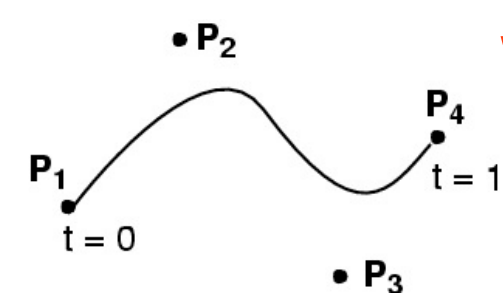
\includegraphics[height=2.5cm]{./slike/bez_obican.png}
		\end{center}
	}
	\only<2-3>{
		\begin{align*}
		\begin{matrix}
		P(u) & = & (1-u)^{3} & P_{1}\\
		& + & 3u(1-u)^{2} & P_{2}\\
		& + & 3u^{2}(1-u) & P_{3}\\
		& + & u^{3} & P_{4}\\
		\end{matrix}
		\end{align*}
		{\color{erlangenlyellow}Promijenili smo $t$ u $u$}}
	
	\only<2>{
		\begin{center}
			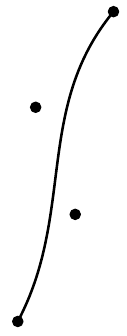
\includegraphics[height=2.5cm]{./slike/bez_surf_01.png}
		\end{center}
	}
	\only<3>{
		\begin{center}
			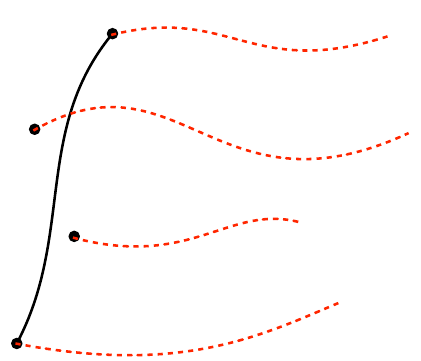
\includegraphics[height=2.5cm]{./slike/bez_surf_02.png}
		\end{center}
	}
	\only<4->{
		\begin{align*}
		\begin{matrix}
		P(u,{\color{erlangenlyellow}v}) & = & (1-u)^{3} & P_{1}{\color{erlangenlyellow}(v)}\\
		& + & 3u(1-u)^{2} & P_{2}{\color{erlangenlyellow}(v)}\\
		& + & 3u^{2}(1-u) & P_{3}{\color{erlangenlyellow}(v)}\\
		& + & u^{3} & P_{4}{\color{erlangenlyellow}(v)}\\
		\end{matrix}
		\end{align*}
		\begin{itemize}
			\item Točke $P$ se gibaju duž krivulja
		\end{itemize}
	}
	\only<4>{
		\begin{center}
			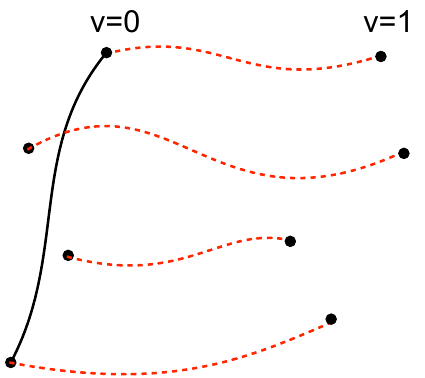
\includegraphics[height=2.5cm]{./slike/bez_surf_03.png}
		\end{center}
	}
	\only<5>{
		\begin{center}
			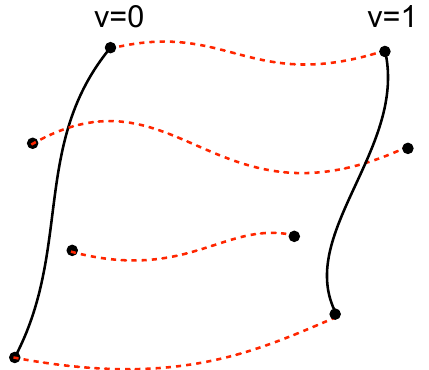
\includegraphics[height=2.5cm]{./slike/bez_surf_04.png}
		\end{center}
	}
	\only<6>{
		\begin{center}
			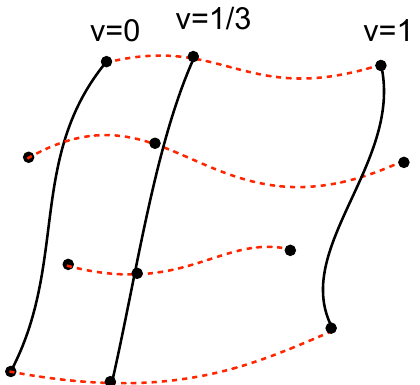
\includegraphics[height=2.5cm]{./slike/bez_surf_05.png}
		\end{center}
	}
	\only<7>{
		\begin{center}
			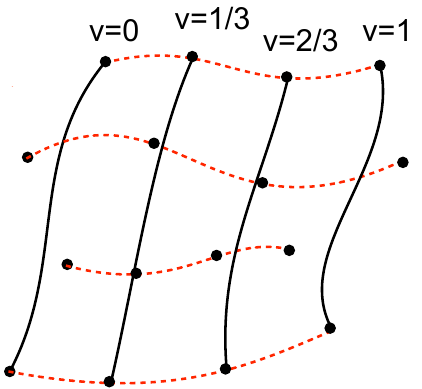
\includegraphics[height=2.5cm]{./slike/bez_surf_06.png}
		\end{center}
	}
	\only<8>{
		\begin{center}
			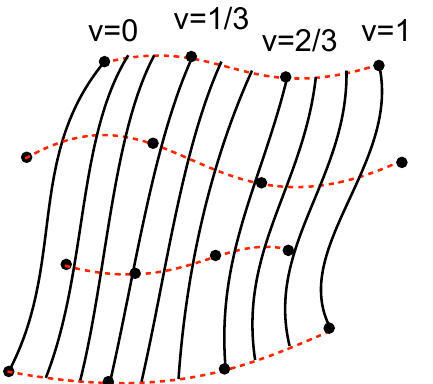
\includegraphics[height=2.5cm]{./slike/bez_surf_07.png}
		\end{center}
	}
	\only<9>{
		\begin{center}
			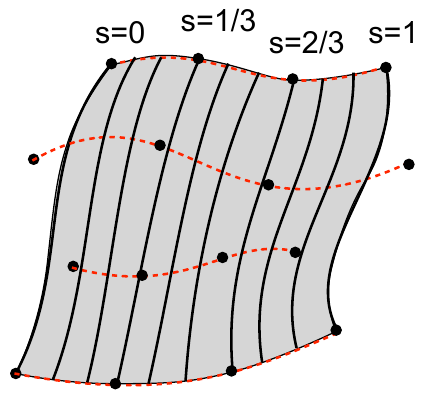
\includegraphics[height=2.5cm]{./slike/bez_surf_08.png}
		\end{center}
	}
	
\end{frame}

\begin{frame}{Prikaz površina}
	\begin{itemize}
		\item<1-> Prijašnji primjer: $P_{i}(v)$ su samo krivulje
		\item<1-> Ako postanu B\`{e}zier krivulje?
		\item<2-> Svaka $u=\mathrm{const.}$ i $v=\mathrm{const.}$ je B\`{e}zierova krivulja
	\end{itemize}
	\only<1>{
		\begin{center}
			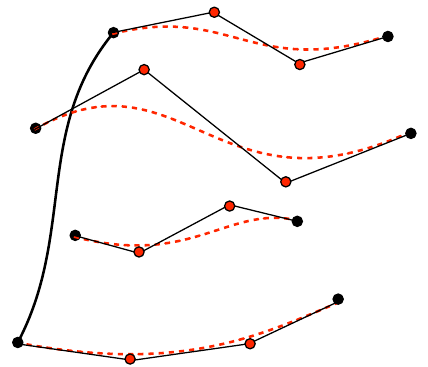
\includegraphics[height=3.cm]{./slike/bez_surf_09.png}
	\end{center}}
	\only<2>{
		\begin{center}
			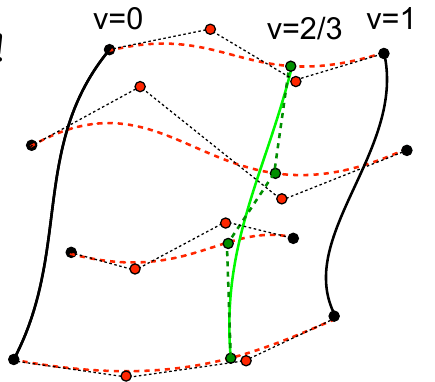
\includegraphics[height=3.cm]{./slike/bez_surf_10.png}
	\end{center}}
\end{frame}

\begin{frame}{Bikubična B\`{e}zierova ploha}
	\only<1>{
		\begin{center}
			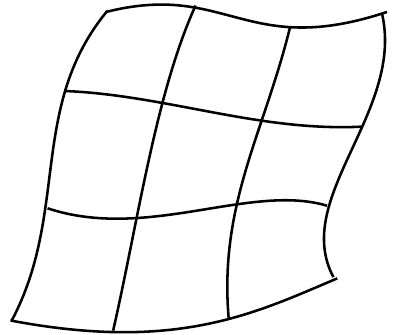
\includegraphics[height=3.cm]{./slike/bez_surf_11.png}
	\end{center}}
	\only<2>{
		\begin{center}
			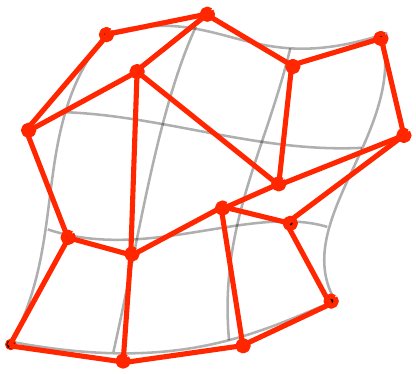
\includegraphics[height=3.cm]{./slike/bez_surf_12.png}
		\end{center}
		\begin{itemize}
			\item interpoliraju se samo četiri rubne krivulje
			\item Kontrolna mreža ima 16 kontrolnih točaka
	\end{itemize}}
\end{frame}

\begin{frame}{Kako računati?}
	\begin{columns}[c]
		\column{.5\textwidth}
		\begin{align*}
		\begin{matrix}
		P(u,v) & = & B_{1}(u) \cdot P_{1}(v)\\
		& + & B_{2}(u) \cdot P_{2}(v)\\
		& + & B_{3}(u) \cdot P_{3}(v)\\
		& + & B_{4}(u) \cdot P_{4}(v)\\
		\end{matrix}
		\end{align*}
		\begin{align*}
		\begin{matrix}
		P_{i}(v) & = & B_{1}(v) \cdot P_{i,1}\\
		& + & B_{2}(v) \cdot P_{i,2}(v)\\
		& + & B_{3}(v) \cdot P_{i,3}(v)\\
		& + & B_{4}(v) \cdot P_{i,4}(v)\\
		\end{matrix}
		\end{align*}
		\column{.5\textwidth}
		\only<1>{
			\begin{center}
				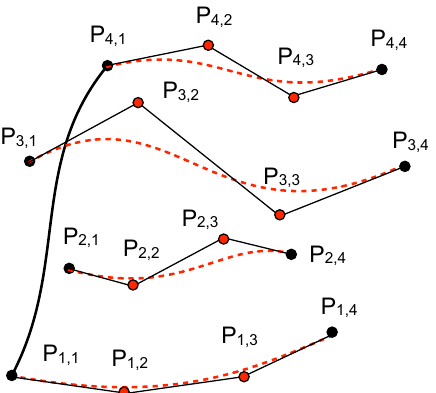
\includegraphics[height=3.cm]{./slike/bez_surf_13.png}
		\end{center}}
		\only<2->{
			\begin{align*}
			P(u,v) & = &  \sum_{i=1}^{4} B_{i}(u)\left(\sum_{j=1}^{4} P_{i,j}B_{j}(v)\right)\\
			& = & \sum_{i=1}^{4} \sum_{j=1}^{4} P_{i,j} B_{i,j}(u,v)
			\end{align*}
			\begin{align*}
			B_{i,j}(u,v) &=& B_{i}(u)\cdot B_{j}(v)
			\end{align*}
			\begin{itemize}
				\item 16 kontrolnih točaka $P_{i,j}$
				\item 16 2D baznih funkcija $B_{i,j}(u,v)$
			\end{itemize}	
		}
	\end{columns}
\end{frame}

\begin{frame}{Kako računati?}
	Matrično:
	\begin{align*}
	P(u,v)  =  \sum_{i=1}^{4} B_{i}(u)\left(\sum_{j=1}^{4} P_{i,j}B_{j}(v)\right)
	\end{align*}
	\begin{align*}
	P(u,v)  =  \mathbf{U}\mathbf{B}\mathbf{P}\mathbf{B}^T\mathbf{V}^T
	\end{align*}
\end{frame}

\begin{frame}{Zaključak, plohe}
	\begin{center}
		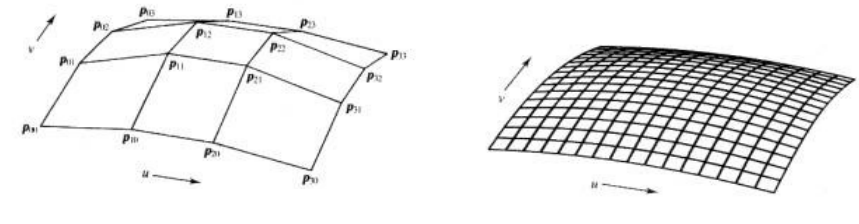
\includegraphics[height=2.cm]{./slike/bez_surf_14.png}
	\end{center}
	\begin{itemize}
		\item Parametarska ploha $P(u,v)$ je kubični polinom dvije varijable, $u$ i $v$
		\item definira se s $4x4=16$ kontrolnih točaka $P_{1,1}, P_{1,2}\ldots P_{4,4}$
	\end{itemize}
\end{frame}

\begin{frame}{Tangente i normale na plohu}
	\begin{itemize}
		\item<1-> $P(u,v)$ je 3D točka određena pomoću $u$ i $v$
		\item<2-> Parcijalne derivacije $\partial P / \partial u$ i  $\partial P / \partial v$ su 3D vektori
		\item<3> Normala je okomita na obje tangente
	\end{itemize}
	\only<3> {$$n = (\partial P / \partial u)\times (\partial P / \partial v)$$}
	\only<1-2>{
		\begin{center}
			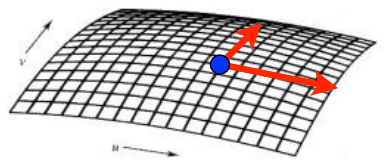
\includegraphics[height=2.cm]{./slike/bez_surf_15.png}
	\end{center}}
	\only<3>{
		\begin{center}
			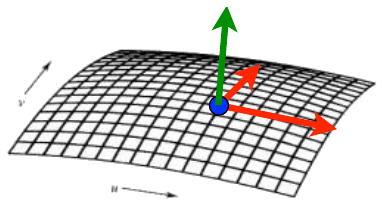
\includegraphics[height=2.cm]{./slike/bez_surf_16.png}
	\end{center}}
\end{frame}

\begin{frame}{Tangente na plohu}
	\begin{align*}
	\vec{t}_u &= \frac{\partial P}{\partial u} \\
	&= \frac{\partial}{\partial u}\left( \mathbf{U}\mathbf{B}\mathbf{P}\mathbf{B}^T\mathbf{V}^T\right) \\
	&= \left(\frac{\partial \mathbf{U}}{\partial u} \mathbf{B}\mathbf{P}\mathbf{B}^T\mathbf{V}^T\right)
	\end{align*}
	Lako je derivirati: za 
	\begin{align*}
	\mathbf{U} = \begin{bmatrix}
	u^3 & u^2  & u& 1 
	\end{bmatrix}
	\end{align*}
	vrijedi
	\begin{align*}
	\frac{\partial \mathbf{U}}{\partial u} = \begin{bmatrix}
	3u^2 & 2u  & 1 & 0 
	\end{bmatrix}
	\end{align*}
\end{frame}

\begin{frame}{Tangente na plohu}
	\begin{align*}
	\vec{t}_v &= \frac{\partial P}{\partial v} \\
	&= \frac{\partial}{\partial v}\left( \mathbf{U}\mathbf{B}\mathbf{P}\mathbf{B}^T\mathbf{V}^T\right) \\
	&= \left(\mathbf{U}\mathbf{B}\mathbf{P}\mathbf{B}^T{\frac{\partial \mathbf{V}}{\partial v}}^T\right)
	\end{align*}
	Lako je derivirati: za 
	\begin{align*}
	\mathbf{V} = \begin{bmatrix}
	v^3 & v^2  & v& 1 
	\end{bmatrix}
	\end{align*}
	vrijedi
	\begin{align*}
	\frac{\partial \mathbf{V}}{\partial v} = \begin{bmatrix}
	3v^2 & 2v  & 1 & 0 
	\end{bmatrix}
	\end{align*}
\end{frame}

\begin{frame}{Normala na plohu}
	\begin{block}{}
		\begin{align*}
		\vec{n} = \vec{t}_u \times \vec{t}_v
		\end{align*}
	\end{block}
	
	\begin{center}
		
\includegraphics[height=4.cm]{./slike/well-duh.jpg}
	\end{center}
\end{frame}	
%\begin{frame}{Intermezzo}
%	\begin{center}
%		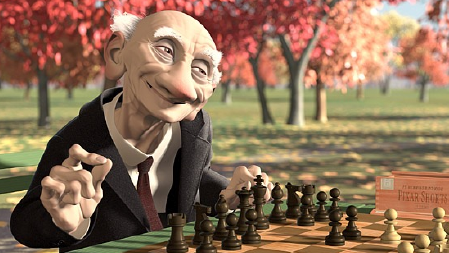
\includegraphics[height=3.cm]{./slike/stari_covjek.png}
%	\end{center}
%\end{frame}

\begin{frame}{Displacement mapping}
	\begin{itemize}
		\item<1-> Nisu sve plohe glatke \ldots
		\item<1-> Obojati plohu s pomacima na glatkoj površini, npr. u smjeru normale
		\item<3-> Glatka ploha postaje mozaik, te se dodaje pomak $D(u,v)$ na vertekse
	\end{itemize}
	\only<1>{
		\begin{center}
			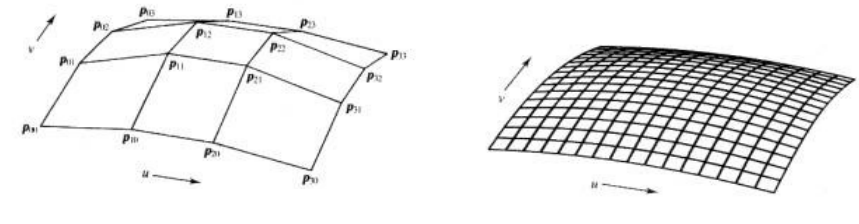
\includegraphics[height=2.cm]{./slike/bez_surf_14.png}
	\end{center}}
	\only<2>{
		\begin{center}
			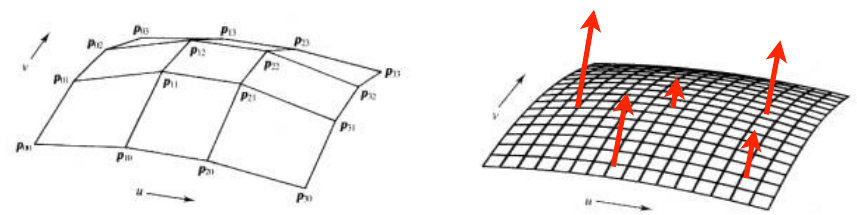
\includegraphics[height=2.cm]{./slike/bez_surf_17.png}
	\end{center}}
\end{frame}
\begin{frame}{Displacement mapping, primjer}
	\begin{center}
		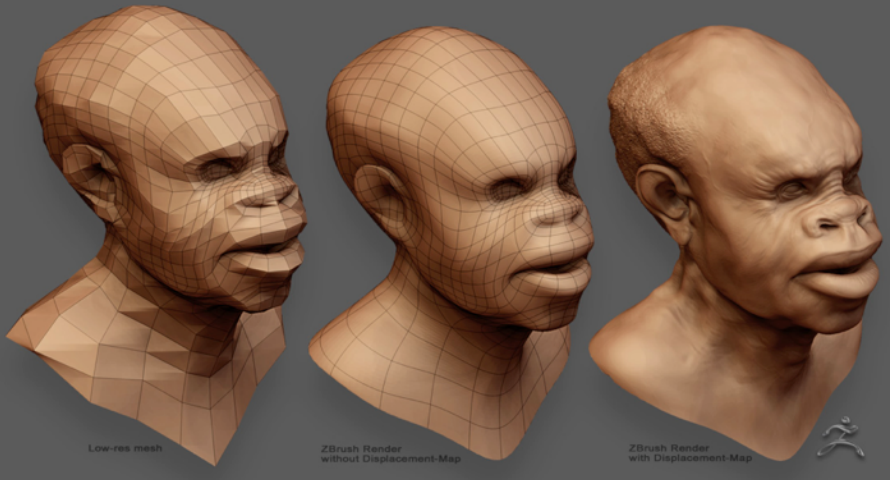
\includegraphics[height=6.cm]{./slike/covjek_displacement.png}
	\end{center}
\end{frame}
\begin{frame}{Ne toliko cool primjene}
	\begin{itemize}
		\item Kreiranje površina rotacijom
		\item generiranje cilindara
	\end{itemize}
	\begin{center}
		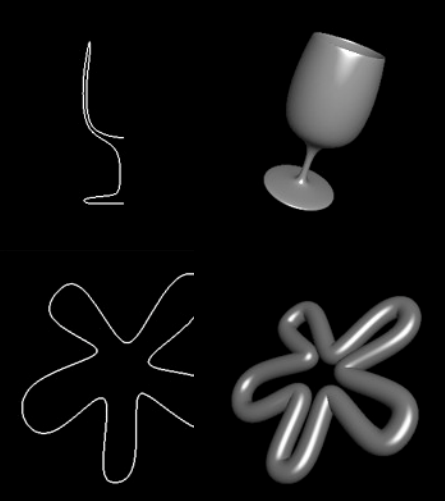
\includegraphics[height=4.cm]{./slike/surface_revolution.png}
	\end{center}
\end{frame}
\begin{frame}{Plohe i rotacija}
	\begin{center}
		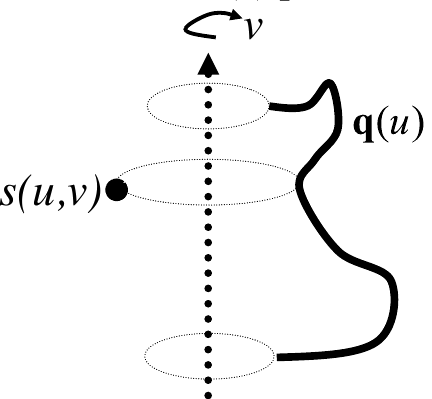
\includegraphics[height=4.cm]{./slike/surface_revolution_02.png}
	\end{center}
\end{frame}

\plain{Pitanja?}
\end{document}